\documentclass{beamer}

\usepackage[utf8]{inputenc}
\usepackage{listings}
\usepackage{xcolor}

\graphicspath{{./images/}}
 
\definecolor{codegreen}{rgb}{0,0.6,0}
\definecolor{codegray}{rgb}{0.5,0.5,0.5}
\definecolor{codepurple}{rgb}{0.58,0,0.82}
\definecolor{backcolour}{rgb}{0.95,0.95,0.92}
 
\lstdefinestyle{mystyle}{
    backgroundcolor=\color{backcolour},   
    commentstyle=\color{violet},
    keywordstyle=\color{red},
    numberstyle=\tiny\color{codegray},
    stringstyle=\color{codegreen},
    basicstyle=\ttfamily\footnotesize,
    breakatwhitespace=false,         
    breaklines=true,                 
    captionpos=b,                    
    keepspaces=true,                 
    numbers=left,                    
    numbersep=5pt,                  
    showspaces=false,                
    showstringspaces=false,
    showtabs=false,                  
    tabsize=2
}
 
\lstset{style=mystyle}


%information to be included in the title page:
\title{JPA Tutorial}
\author{Adriano Botti, Antonio Le Caldare, Francesco Merola, Giacomo Ponziani}
\institute{Information Systems, University of Pisa}
\date{Fall, 2019}

\begin{document}

%generates the title page containing introductory information
\frame{\titlepage}

\begin{frame}
\frametitle{What is and Why JPA}
JPA (Java Persistence API) is a Java specification for ORM (Object Relational Mapping). The purpose of ORM is to map the concepts from ObjectOriented Programming with concepts of relational databases to let the programmer to focus on the business logic instead of the translation between the two worlds. Once the mapping is done it is possble to work with instances of classes that are directly mapped to rows of table without performing any transformation.
In this tutorial we focus on Hibernate which is one of the implementation of the JPA specification. 
\end{frame}

\begin{frame}
\frametitle{How to use JPA}
Mapping may be done using \textit{annotations} or \textit{persistence.xml} file or both. Usually the \textit{persistence.xml} file is used to store information about the connection with the DB while \textit{annotations} are used actually map classes into tables.
\begin{enumerate}
\item Define the \textit{persistence.xml} file;
\item Define classes using private fields with getter and setter methods and \textit{annotations} to map them with tables;
\item Use \textit{JPQL} to perform \textit{CRUD} operations;
\end{enumerate}
\end{frame}

\begin{frame}
\frametitle{Examples Definition}
All the following examples come from the application developed in \textit{Task 1}. This application handles university exams creation, registration, deregistration and validation.
For clarity the class-diagram is reported.
\linebreak
\begin{figure}
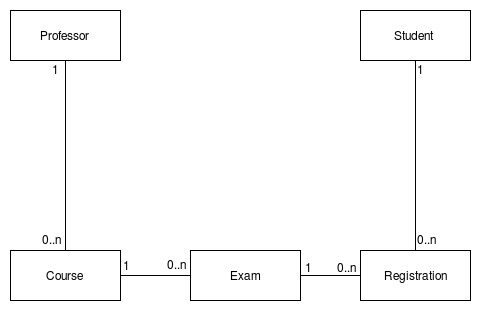
\includegraphics[scale=0.45]{ClassDiagram.png}
\centering
\end{figure}
\end{frame}

\begin{frame} [fragile]
\frametitle{JPA Annotations}
\begin{itemize}
\item \textit{@Entity}, specifies the following class is an entity to be mapped to one or more tables in the DB.
\item \textit{@Table}, specifies the primary table for the annotated entity. The attribute \textit{name} indicates the referenced table in the DB.
\item \textit{@Column}, specifies the mapped column for a persistent property or field. The attribute \textit{name} indicates the name of the corresponding table column. It may be neglected when names of the attribute and of the columns are the same.
\end{itemize}
\begin{lstlisting}[language=Java, caption=@Entity and @Table]
@Entity
@Table(name = "professor")
public class Professor {...}
	
\end{lstlisting}
\end{frame}

\begin{frame}[fragile]
	\frametitle{JPA Annotations}
	Annotation may be before a field or a method but not both. In the case the annotation is before the method
	\begin{itemize}
		\item \textit{@Id}, specifies the primary key for an entity. The class of the primary key shall implement \textit{Serializable} interface and the \textit{equal} and \textit{hash} methods.
	\end{itemize}
	\begin{lstlisting}[language=java, caption=@Id @Column and @GeneratedValue]
		@Column(name = "id")
		@Id
		@GeneratedValue(strategy = GenerationType.IDENTITY)
		public int getId() {
		return id;
		}
	\end{lstlisting}
\end{frame}

\begin{frame} [fragile]
	\frametitle{JPA ANNOTATIONS}
	\begin{itemize}
		\item \textit{@Embeddable}, before a class definition indicates that the class can be included into another one tagged with \textit{@Entity}. The Embeddable class cannot be mapped to a db table alone as it represents only a portion of it.
		\begin{lstlisting} [language=java, caption=@Embeddable]
@Embeddable
public static class RegistrationId implements Serializable {
	private int student;
	private Exam.ExamID exam;
	
	public RegistrationId() {...}	
	public int getStudent() {...}
	public void setStudent(int student) {...}
	public Exam.ExamID getExam() {...}
	public void setExam(Exam.ExamID exam) {...}
		
	@Override
	public boolean equals(Object obj) {...}		
	@Override
	public int hashCode() {...}
}
		\end{lstlisting}
	\end{itemize}
\end{frame}

\begin{frame} [fragile]
	\frametitle{JPA ANNOTATIONS}
	\begin{itemize}
		\item \textit{@EmbeddedId}, indicates that the primary key of the class is composite and that it is an \textit{@Embeddable} class. In this case the get method specifies that \textit{id} is the primary key.
	\end{itemize}
	\begin{lstlisting} [language=java, caption=@EmbeddedId]
@Entity
@Table(name = "exam_result")
public class Registration {
	private RegistrationId id;
	\*...*\
	@EmbeddedId
	public RegistrationId getId() {...}
	\*...*\
}
	\end{lstlisting}
\end{frame}

\begin{frame} [fragile]
	\frametitle{JPA ANNOTATIONS}
	\begin{itemize}
		\item \textit{@ManyToOne} specifies a many to one relationship with another class. The target entity is inferred from the type of the object being referenced. The target is expeted to have a \textit{OneToMany} annotation only if the application logic requires it, indeed in this application the \textit{Student} class does not have such annotation since it is required to get the students data from registration and not viceversa.
		\item \textit{@MapsId} states the next \textit{@ManyToOne} (it can also be \textit{@OneToOne}) relationship maps an attribute within the \textit{EmbeddedId} with an attribute of another class specified with the get method: in this case \textit{student} attribute of the embedded class is map to the \textit{id} attribute of the \textit{Student} class.
	\end{itemize}
	\begin{lstlisting} [language=java, caption=Foreign key]
@MapsId("student")
@JoinColumn(name="student", referencedColumnName="id")
@ManyToOne
public Student getStudent () {...}\end{lstlisting}
\end{frame}

\begin{frame} [fragile]
	\frametitle{JPA ANNOTATIONS}
	\begin{itemize}
		\item \textit{@JoinColumn} specifies a column for joining.
	\end{itemize}
	\begin{lstlisting}[language=java, caption=Foreign key]
@MapsId("exam")
@JoinColumns({
	@JoinColumn(name="course", referencedColumnName="course"),
	@JoinColumn(name="date", referencedColumnName="date")
})
@ManyToOne
public Exam getExam() {...}
public void setExam(Exam exam) {...}\end{lstlisting}
This is another example of foreign key: the attribute \textit{exam} of the \textit{Embeddable} class \textit{RegistrationId} is mapped to the \textit{Exam} class thorough the attributes \textit{course} and \textit{date}.
\end{frame}


\begin{frame} [fragile]
\begin{itemize}
\frametitle{JPA ANNOTATIONS}
\item @ManyToMany, specifies a many-valued association with many-to-many multiplicity.  If for example we change our application and we suppose that more than one professor can teach a course we have a many to many relationship between the two entities. We suppose that the courses are more used in our application and therefore makes sense to set \textit{Course} entity as the \textit{owning side} using the \text{@JoinTable}: it specifies the name of the joining table and joining columns.
\end{itemize}
\end{frame}

\begin{frame} [fragile]
\frametitle{JPA ANNOTATIONS}
\begin{lstlisting} [language=java, caption=@ManyToMany Professor]
@Entity
@Table(name="Professor")
public class Professor {
	/*
	 *
	 */
	 private Collection<Course> courses = new Collection<>();
	 @ManyToMany(mappedBy=professors)
	 //mappedBy indicates the attribute in the owning side
	 public Collection<Course> getCourses(){ return courses; }
	 /*
	  *
	  */
}
\end{lstlisting}
\end{frame}

\begin{frame} [fragile]
\frametitle{JPA ANNOTATIONS}
\begin{lstlisting} [language=java, caption=@ManyToMany Course]
@Entity
@Table(name="Course")
public class Course {
	/*
	 *
	 */
	 private Collection<Professor> professors = new Collection<>();
	 @ManyToMany
	 @JoinTable {
	 	name = "Course_Professors",
	 	joinColumns = {@JoinColumn(name="professor_id")},
	 	inverseJoinColumns = {@JoinColumn(name="course_id")}
	 }
	 public Collection<Professor> getProfessors() { return professors; }
	 /*
	  *
	  */
}
\end{lstlisting}
\end{frame}

\begin{frame}
	\frametitle{JPQL - Introduction}
	The Java Persistence Query Language (JPQL) is a platform-independent object-oriented query language defined as part of the Java Persistence API (JPA) specification.
	\linebreak
	\linebreak
	JPQL is used to make queries against entities stored in a relational database. It is heavily inspired by SQL, and its queries resemble SQL queries in syntax, but operate against JPA entity objects rather than directly with database tables.
\end{frame}

\begin{frame} [fragile]
\frametitle{JPQL - Read}
Given a student id (\textit{studId}) find the exams the student has not yet passed.
\begin{lstlisting}[language=sql]
SELECT e
FROM Exam e
WHERE (SELECT count(r)
	FROM Registration r
	WHERE r.student.id = :studId AND
	      --studId is a parameter
	      r.exam.id = e.id OR
	      (r.exam.course = e.course AND r.grade IS NOT NULL)) = 0);
\end{lstlisting}
\end{frame}

\begin{frame} [fragile]
\frametitle{JPQL - Create}
Insert a new registration: first we obtain the corresponding student and exam and then we create a new registration.
\begin{lstlisting} [language=java]
public void insertRegistration(int studentId, Exam examDetached, @Nullable Integer grade){
	/***/
	entityManager = factory.createEntityManager();
	
	Student student = entityManager.getReference(Student.class, studentId);
	Exam exam = entityManager.getReference(Exam.class, examDetached.getId());
	Registration registration = new Registration(student, exam, grade);
	
	entityManager.getTransaction().begin();
	entityManager.persist(registration);
	entityManager.getTransaction().commit();
	/***/
}
\end{lstlisting}
\end{frame}

\begin{frame} [fragile]
\frametitle{JPQL - Update}
Update an existing registration inserting the grade.
\begin{lstlisting} [language=java]
public void updateRegistration(Registration reg, int grade) {
	reg.setGrade(grade);
	try {
		entityManager = factory.createEntityManager();
		entityManager.getTransaction().begin();
		entityManager.merge(reg);
		entityManager.getTransaction().commit();
	} catch (Exception ex) {
		ex.printStackTrace();
		System.out.println("A problem occurred inserting a registration!");
		throw ex;
	} finally {
		entityManager.close();
	}
}
\end{lstlisting}
\end{frame}

\begin{frame} [fragile]
\frametitle{JPQL - Delete}
Delete a registration.
\begin{lstlisting} [language=java]
public void deleteRegistration(int studentId, Exam exam) {
	try {
		entityManager = factory.createEntityManager();
		entityManager.getTransaction().begin();
		Query query = entityManager.createQuery("DELETE FROM Registration r WHERE r.exam = :exam AND r.student.id = :studId");
		query.setParameter("exam", exam);
		query.setParameter("studId", studentId);
		query.executeUpdate();
		entityManager.getTransaction().commit();
	} catch (Exception ex) {
		ex.printStackTrace();
		System.out.println("A problem occurred inserting a registration!");
		throw ex;
	} finally {
		entityManager.close();
	}
}

\end{lstlisting}
\end{frame}

\end{document}
